\section{Experiments}
\label{sec:Experiments}
While the exact performance of the \tagName system will be implementation dependant i.e. different size/shape magnets, encoder ICs, etc... we performed two categories of experimentation to demonstrate that our implementation of the \tagName concept is feasible and useful in the context of modular robots. The first section~\ref{sec:characterize} attempts to characterize the \tagNamePlural in terms of repeatability and accuracy of multiple measurements under varying conditions and to investigate the behavior when tags are misaligned. The second section~\ref{sec:mblocksExperiments} illustrates the use of the \tagNamePlural implemented on a system consisting of 8 active 3D M-Blocks modular robots, in addition to numerous passively tagged modules.

\begin{figure}[ht]

	%% Figure of electronics Diagram
\tikzset{box/.style={draw, rectangle, rounded corners, thick, node distance=7em, text width=6em, text centered, minimum height=3.5em}}
\tikzset{container/.style={draw, rectangle, rounded corners, dashed, inner sep=1em}}
\tikzset{line/.style={draw, thick, -latex'}}

\begin{tikzpicture}[auto]
	\node[anchor=south west,inner sep=0, minimum width = \linewidth, minimum height = 8.5cm] (emptyBox) at (0,0) {};
	\begin{scope}[x={(emptyBox.south east)},y={(emptyBox.north west)}]
	\tikzset{>=latex}
		\coordinate (leftCenter) at (0.12, 0.75);
		\coordinate (rightCenter) at (0.6, 0.85);
		\coordinate (routePt) at (0.50, 0.75);
		
		% Main Board
		\node [box] (mainBoard) at (leftCenter) {High Level Control Board (ESP8266)};
		
		% Kyles Boards...
	%	\node [box] at ([shift = ({225:3.5 cm})] mainBoard) (kb) {Motor and Power Board (nRF51422)};
	%	\node [box, right = 1.5cm of kb] (db)  {Actuator Control Board};
		
		% Face Boards
		\node [box] (f0) at (rightCenter) {Face 0 PCB  (IO~Expander)};
		\node [box, below = 0.25cm of f0] (f1) {Face 1 PCB   (IO~Expander)};
		\node [below = 0.75cm of f1] (f2) {...};
		\node [box, below = 0.75cm of f2] (f5) {Face 5 PCB   (IO~Expander)};
		
		%% I2C Connections
		\path [line, <->, orange, ultra thick] (mainBoard) -- (routePt)-- (f0);
		\path [line, <->, orange, ultra thick] (mainBoard) -- (routePt)-- (f1);
		\path [line, <->, orange, ultra thick] (mainBoard) -- (routePt)-- (f5);
		
	%	\path [line, <->, orange, ultra thick] (kb) -- (db);
		
		%% Serial Connections
		
	%	\path [line, <->, blue, ultra thick] (kb) -- (mainBoard);

		%% Inputs
		\node [align = center] (input1) at (0.91, 0.45) {Environmental \\ and \\ Neighbor \\ sensing};
	%	\node [align = left] (input2) at (0.16, 0.96) {wifi commands};

	%	\node [align = left] (input3) at (0.25, 0.24) {Motor \\ Batteries \\ SMA wire};
	%	\node [align = left] (input4) at (0.4, 0.24) {Brake \\ Em coil};
		
%		\draw [dashed,  <->] (kb.south) to [out = 270, in = 180] (input3.west);
%		\draw [dashed,  <->] (input2.south) to [out = 270, in = 235] (mainBoard.west);
%		\draw [dashed,  <->] (input4.east) to [out = 0, in = 325] (db.east);
		
		\draw [dashed,  ->] (input1.north) to [out = 90, in = 0] (f0.east);
		\draw [dashed,  ->] (input1.north) to [out = 90, in = 0] (f1.east);
		\draw [dashed,  ->] (input1.south) to [out = 270, in = 0] (f5.east);
		
		% Dashed Boxes
	%	\node[container, fit = (mainBoard) (kb) (db) (input4) (input3)] (core) {};
	%	\node at (core.south) [below, node distance = 0 and 0] {\textbf{Core}};

		\node[container, fit = (f0) (f5)] (frame) {};
		\node at (frame.south) [below, node distance = 0 and 0] {\textbf{Frame}};

%    	\node [box] (planning) {Planning};
%   	 	\node [box, below of=planning, maroon, inner sep = 0pt] (resources) {Resources};
%   	 	\node [box, below of=resources] (sensors) {Sensors};
%    	\node [box, below of=sensors] (processing) {Processing};
%    	\node [box, below of=sensors] (processing) {Processing};
%    	\node [box, below of=sensors] (processing) {Processing};
%
%    	\coordinate (middle) at ($(resources.west)!0.5!(sensors.west)$);
%    	\node [box, above of=middle, node distance=4 cm] (archive) {Archive};
%    	\node [box, below of=archive, node distance=4 cm] (reporting) {Reporting};
%
%    	\node[container, fit=(resources) (sensors)] (or) {};
%    	\node at (or.north west) [above right,node distance=0 and 0] {OR};
%
%	    \node[container, fit=(archive) (reporting)] (his) {};
%    	\node at (his.north west) [above right,node distance=0 and 0] {HIS};
%
%    	\path [line, line width = 0.5mm, red] (planning) -- (resources);
%    	\path [line] (resources) -- (sensors);
%    	\path [line] (sensors) -- (processing);
%
%    	\path [line] (archive) |- (planning);
%    	\path [line] (archive) |- (processing);
%    	\path [line] (processing)--($(processing.south)-(0,0.5)$) -| (reporting);
%
%    	\draw [line] ($(processing.south)-(0,0.5)$) -- ++(4,0) node(lowerright){} |- (planning.east);
%    	\draw [line] (lowerright |- or.east) -- (or.east -| resources.south east);
%
%    	\draw[line] (archive.170)--(reporting.10);
%    	\draw[line] (reporting.350)--(archive.190);
    \end{scope}
\end{tikzpicture}


%
%
%	\begin{tikzpicture}
%	\node[anchor=south west,inner sep=0] (image) at (0,0) {\includegraphics[width=0.9\textwidth]{some_image.jpg}};
%	\begin{scope}[x={(image.south east)},y={(image.north west)}]
%
%	\end{scope}
%	\end{tikzpicture}
%\end{document}
	
	
	\caption{System diagram for implementing the algorithms}
	
	\label{fig:PlaneChanging2}
\end{figure}



%%%%%%%%%%%%%%%%%%%%%%%%%%%%%%%%%%%%%%%%%%%%%%%%%%%%%%%%%%%%%%%%%%%%%%%%%%%%%%%%%%%%%%%%%%%%%%%%%%%%%%%%%%%%%%%%%%%%%%%%%%%%%%%%%%%%%%%%%%%%%%%
%%%%%%%%%%%%%%%%%%%%%%%%%%%%%%%%%%%%%%%%%%%%%%%%%%%%%%%%%%%%%%%%%%%%%%%%%%%%%%%%%%%%%%%%%%%%%%%%%%%%%%%%%%%%%%%%%%%%%%%%%%%%%%%%%%%%%%%%%%%%%%%
\subsection{Arrow Following experiments}
\label{sec:mblocksExperimentsArrow}
%%%%%%%%%%%%%%%%%%%%%%%%%%%%%%%%%%%%%%%%%%%%%%%%%%%%%%%%%%%%%%%%%%%%%%%%%%%%%%%%%%%%%%%%%%%%%%%%%%%%%%%%%%%%%%%%%%%%%%%%%%%%%%%%%%%%%%%%%%%%%%%
%%%%%%%%%%%%%%%%%%%%%%%%%%%%%%%%%%%%%%%%%%%%%%%%%%%%%%%%%%%%%%%%%%%%%%%%%%%%%%%%%%%%%%%%%%%%%%%%%%%%%%%%%%%%%%%%%%%%%%%%%%%%%%%%%%%%%%%%%%%%%%%
We 

\begin{table}[h]
	\caption{Experimental results for }
	
	\begin{tabular}{ p{3.4cm}  p{1.9cm}  p{1.9cm} }
		\hline
								& Attempts 	& Successes \\
		\hline
		Configuration Discovery	&  -1 		& -50 \\
		Direction Following		& 0 		& 0  \\
		command Tags 			&  -1 		& -50 \\		
	\end{tabular}
	
	\label{tab:info}
\end{table}

%%%%%%%%%%%%%%%%%%%%%%%%%%%%%%%%%%%%%%%%%%%%%%%%%%%%%%%%%%%%%%%%%%%%%%%%%%%%%%%%%%%%%%%%%%%%%%%%%%%%%%%%%%%%%%%%%%%%%%%%%%%%%%%%%%%%%%%%%%%%%%%
%%%%%%%%%%%%%%%%%%%%%%%%%%%%%%%%%%%%%%%%%%%%%%%%%%%%%%%%%%%%%%%%%%%%%%%%%%%%%%%%%%%%%%%%%%%%%%%%%%%%%%%%%%%%%%%%%%%%%%%%%%%%%%%%%%%%%%%%%%%%%%%
\subsection{line formation experiments}
\label{sec:mblocksExperimentsLine}
%%%%%%%%%%%%%%%%%%%%%%%%%%%%%%%%%%%%%%%%%%%%%%%%%%%%%%%%%%%%%%%%%%%%%%%%%%%%%%%%%%%%%%%%%%%%%%%%%%%%%%%%%%%%%%%%%%%%%%%%%%%%%%%%%%%%%%%%%%%%%%%
%%%%%%%%%%%%%%%%%%%%%%%%%%%%%%%%%%%%%%%%%%%%%%%%%%%%%%%%%%%%%%%%%%%%%%%%%%%%%%%%%%%%%%%%%%%%%%%%%%%%%%%%%%%%%%%%%%%%%%%%%%%%%%%%%%%%%%%%%%%%%%%

\begin{figure}[h]  
	\centering
	\begin{subfigure}[b]{0.3\linewidth}
		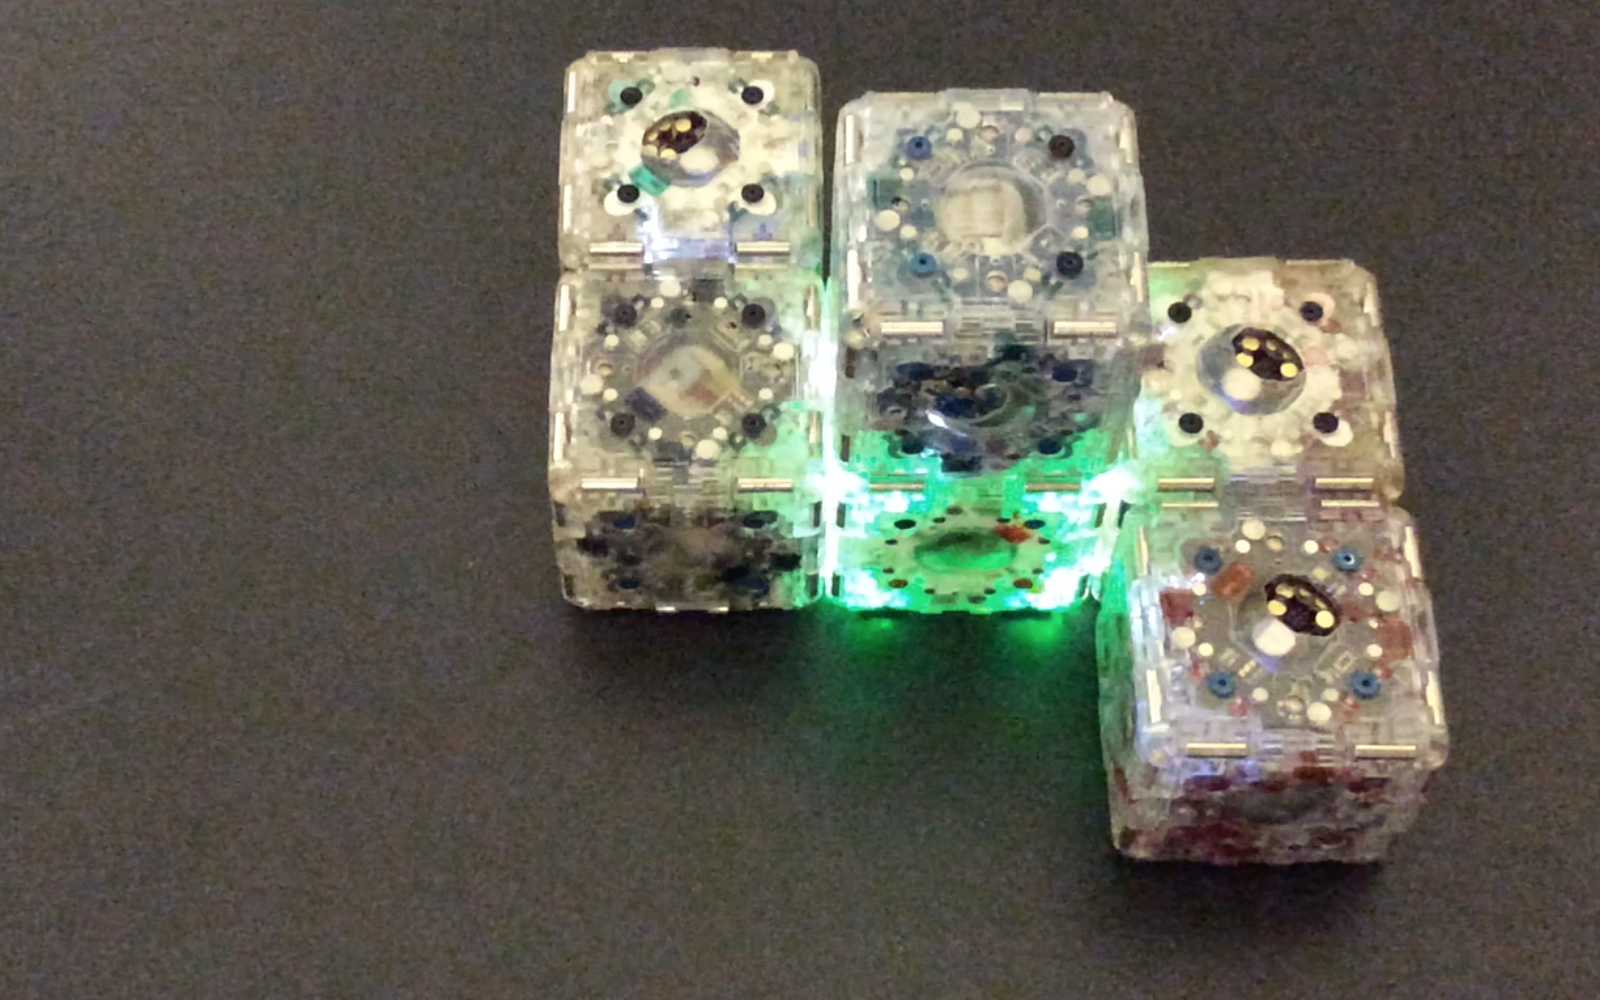
\includegraphics[width=0.9\linewidth]{figures/ActualLine_1.png}
		\subcaption{} 
	\end{subfigure}
	\begin{subfigure}[b]{0.3\linewidth}
		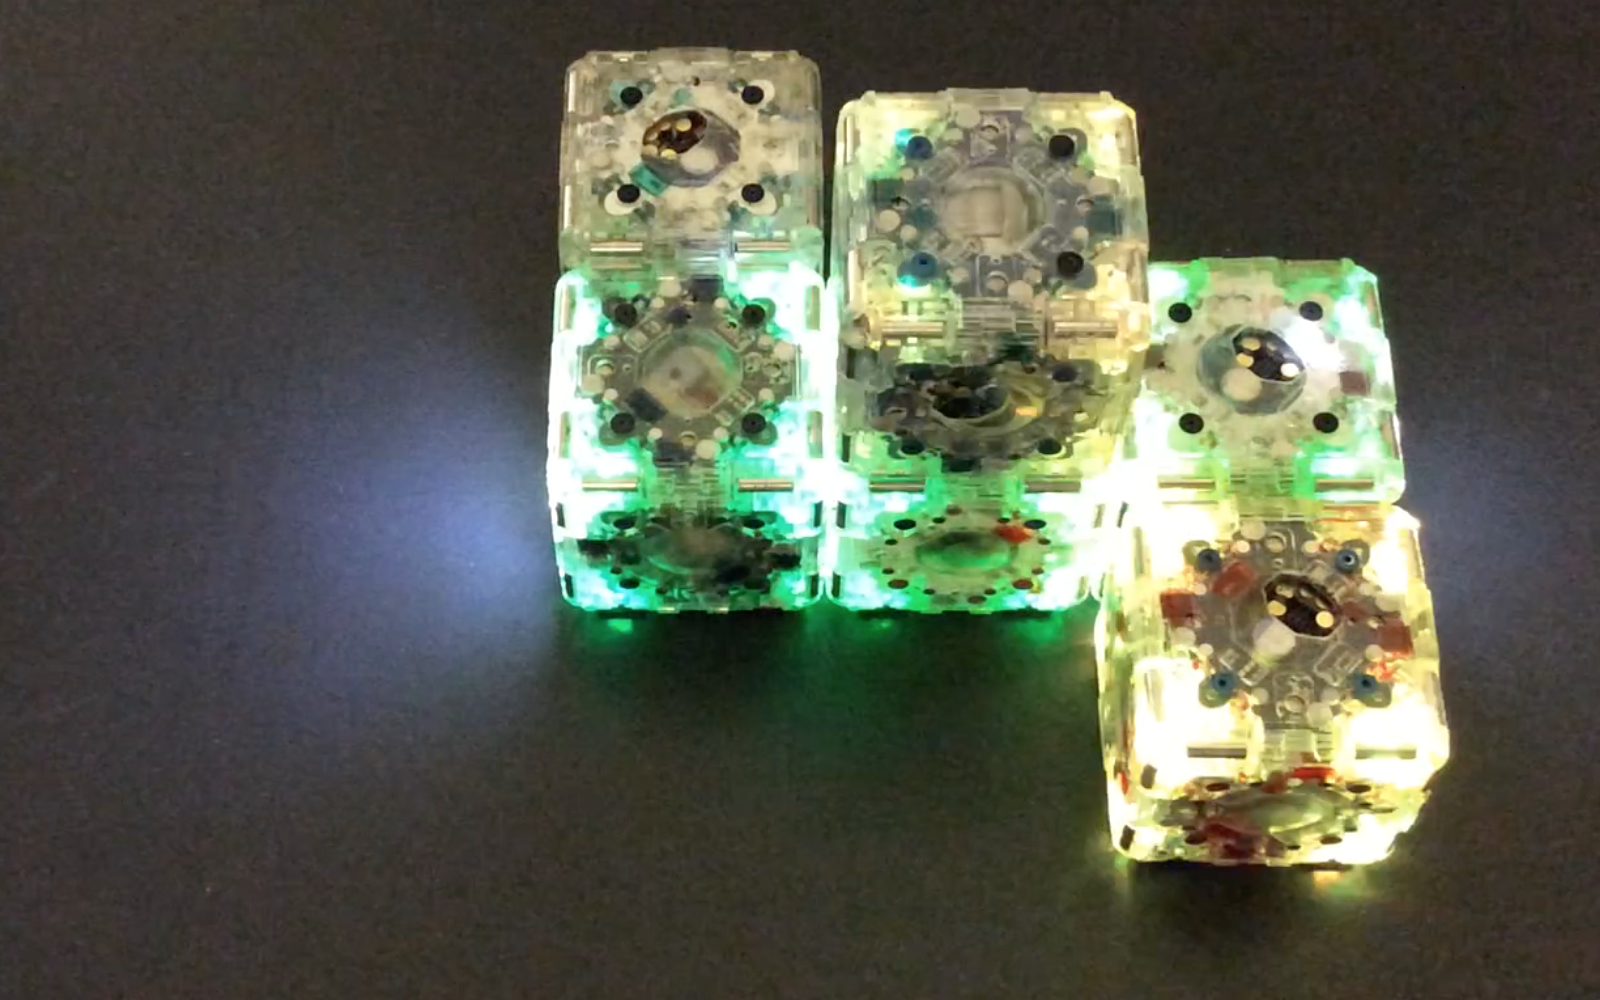
\includegraphics[width=0.9\linewidth]{figures/ActualLine_2.png}
		\subcaption{} 
	\end{subfigure}
	\begin{subfigure}[b]{0.3\linewidth}
		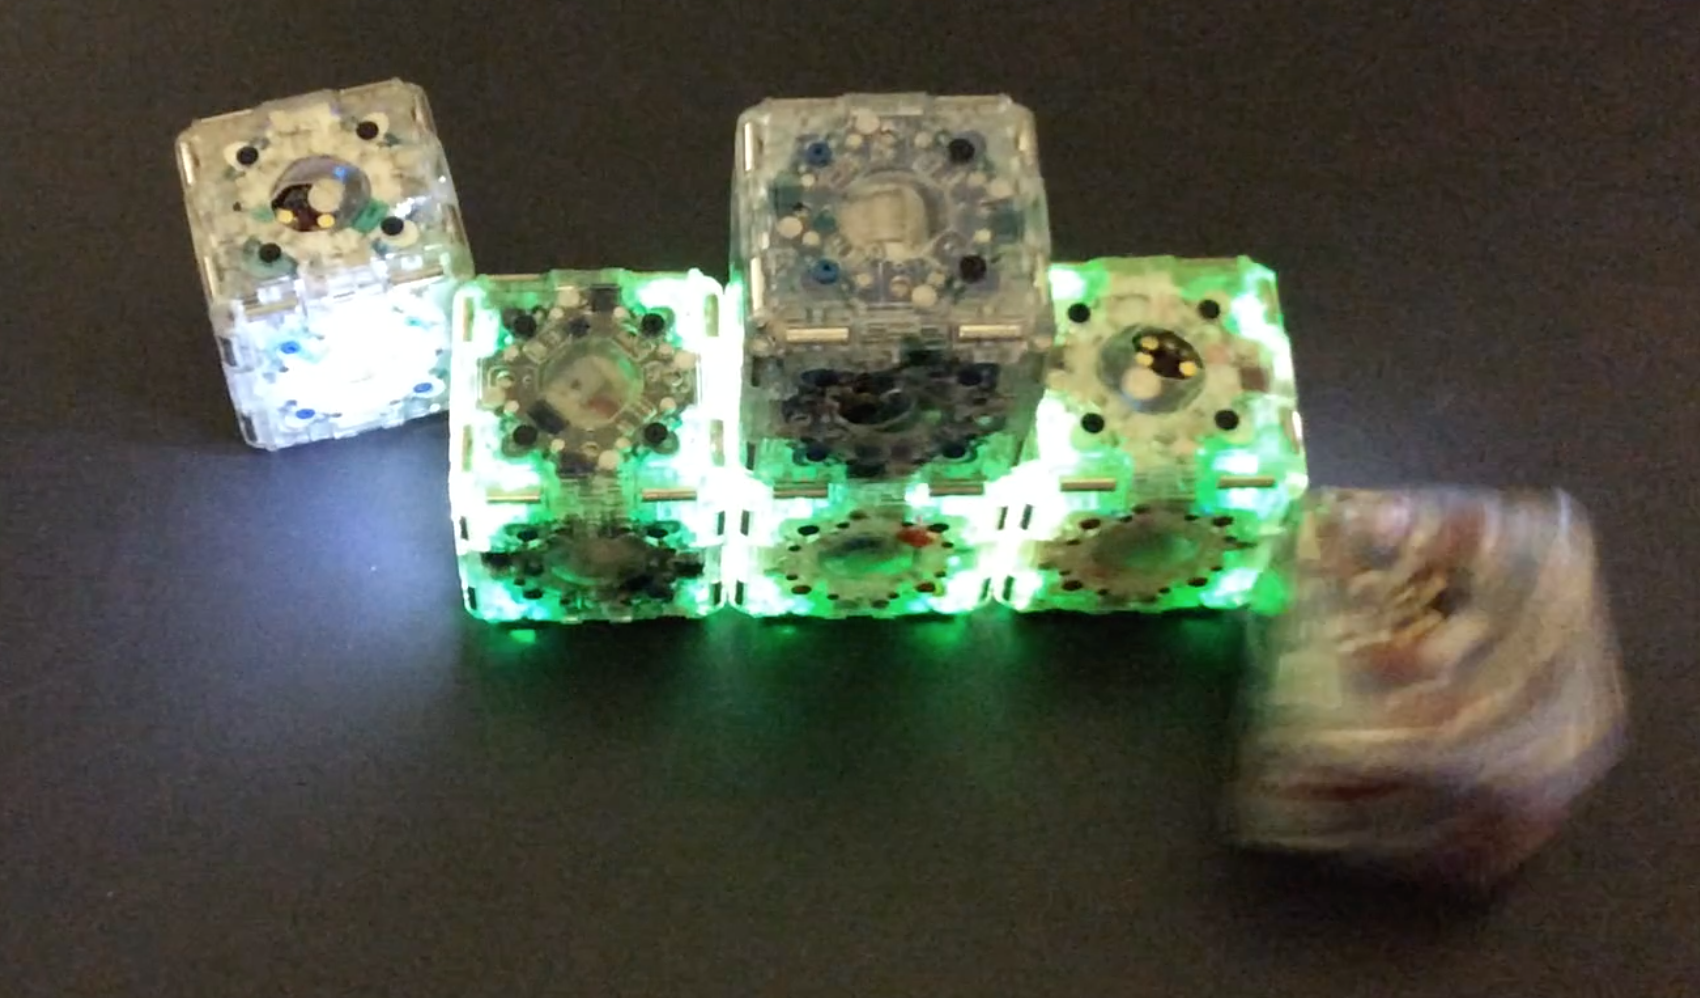
\includegraphics[width=0.9\linewidth]{figures/ActualLine_3.png}
		\subcaption{} 
	\end{subfigure}

	\begin{subfigure}[b]{0.3\linewidth}
		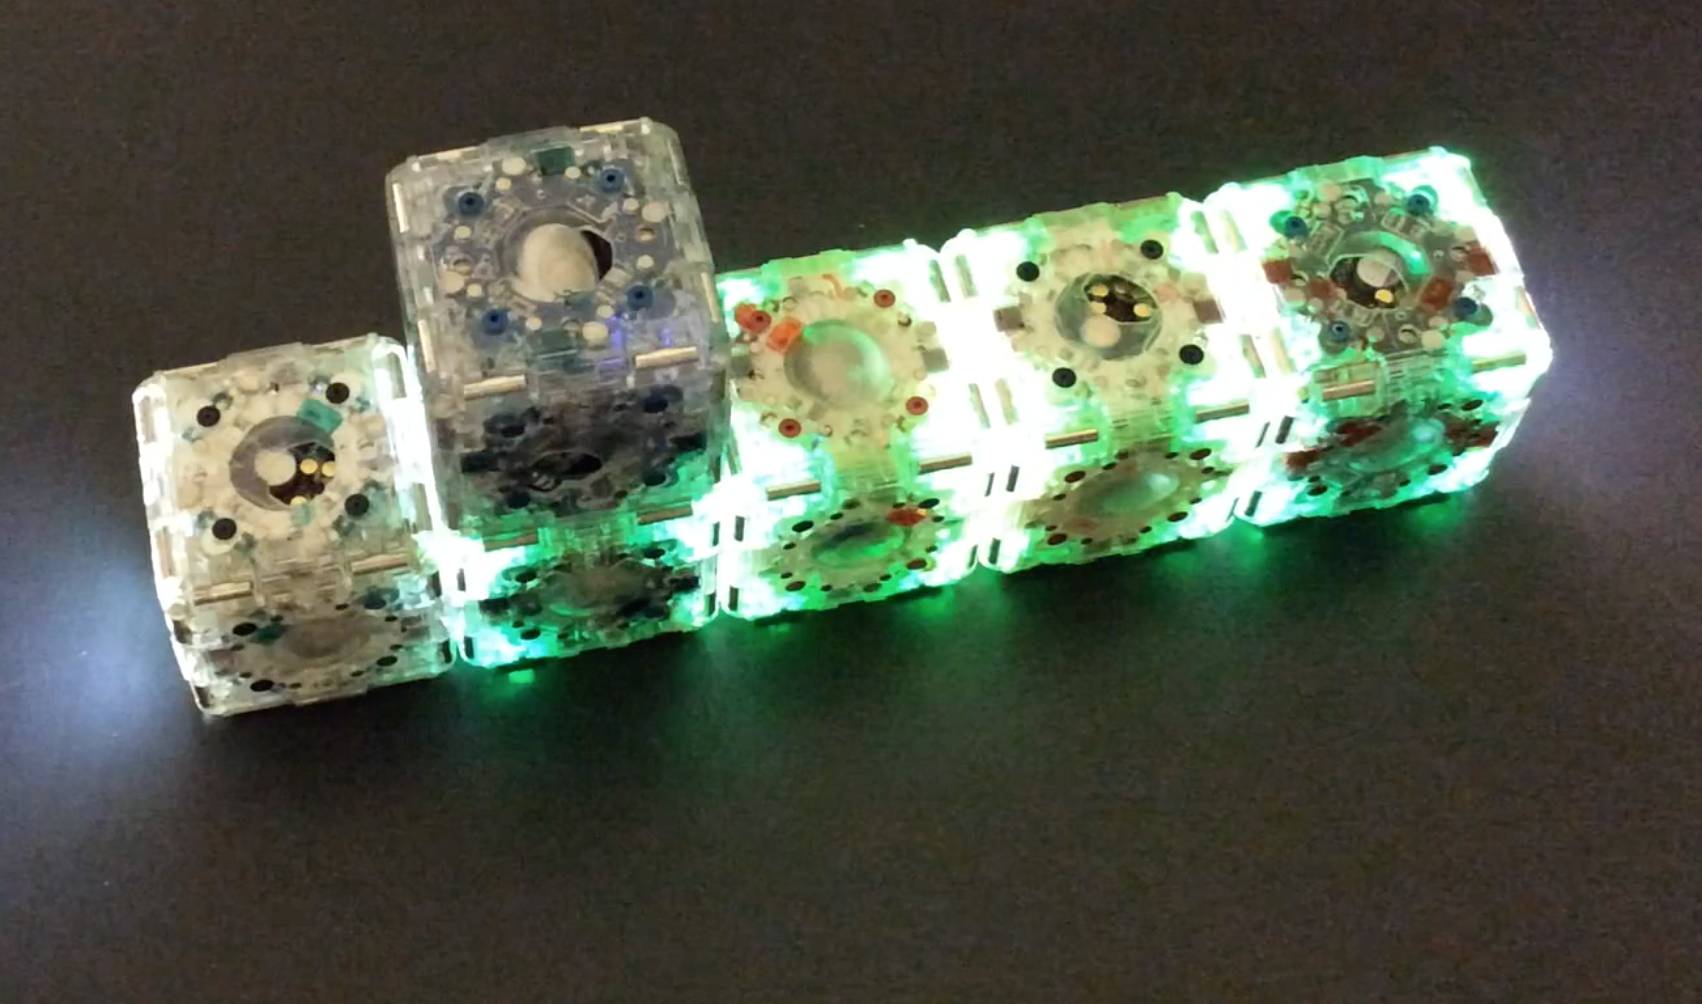
\includegraphics[width=0.9\linewidth]{figures/ActualLine_4.png}
		\subcaption{} 
	\end{subfigure}
	\begin{subfigure}[b]{0.3\linewidth}
		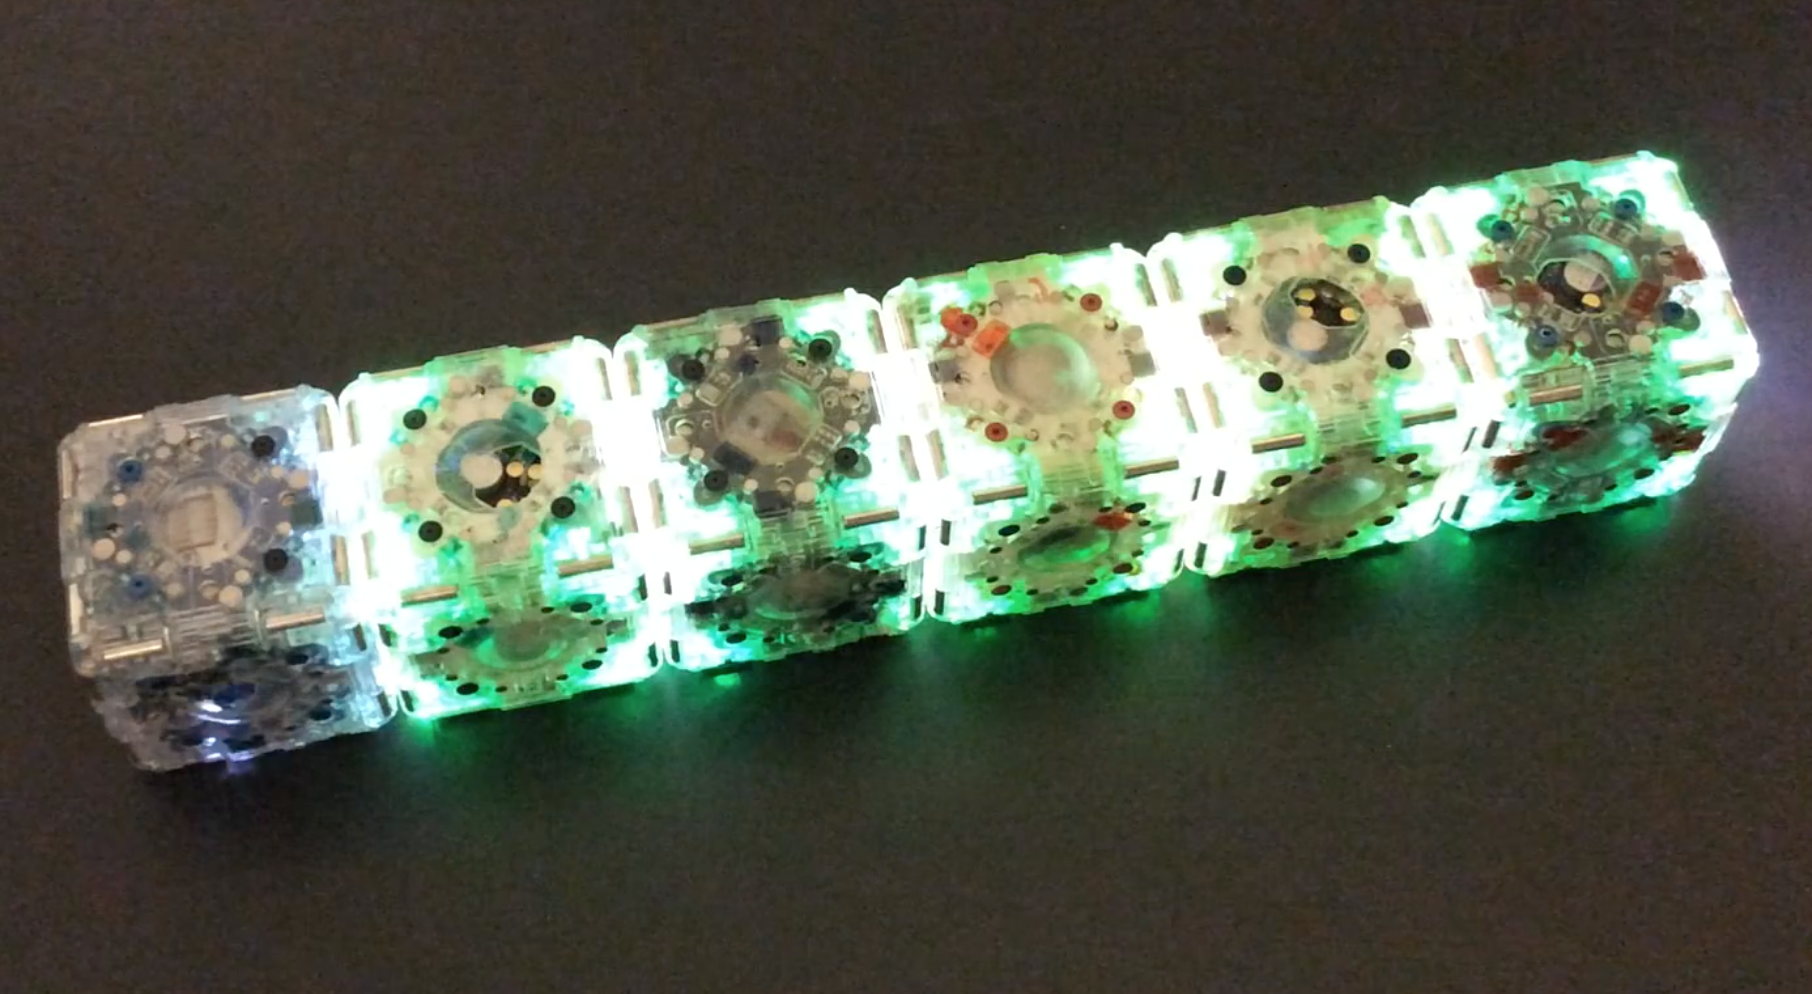
\includegraphics[width=0.9\linewidth]{figures/ActualLine_5.png}
		\subcaption{} 
	\end{subfigure}
	\begin{subfigure}[b]{0.3\linewidth}
		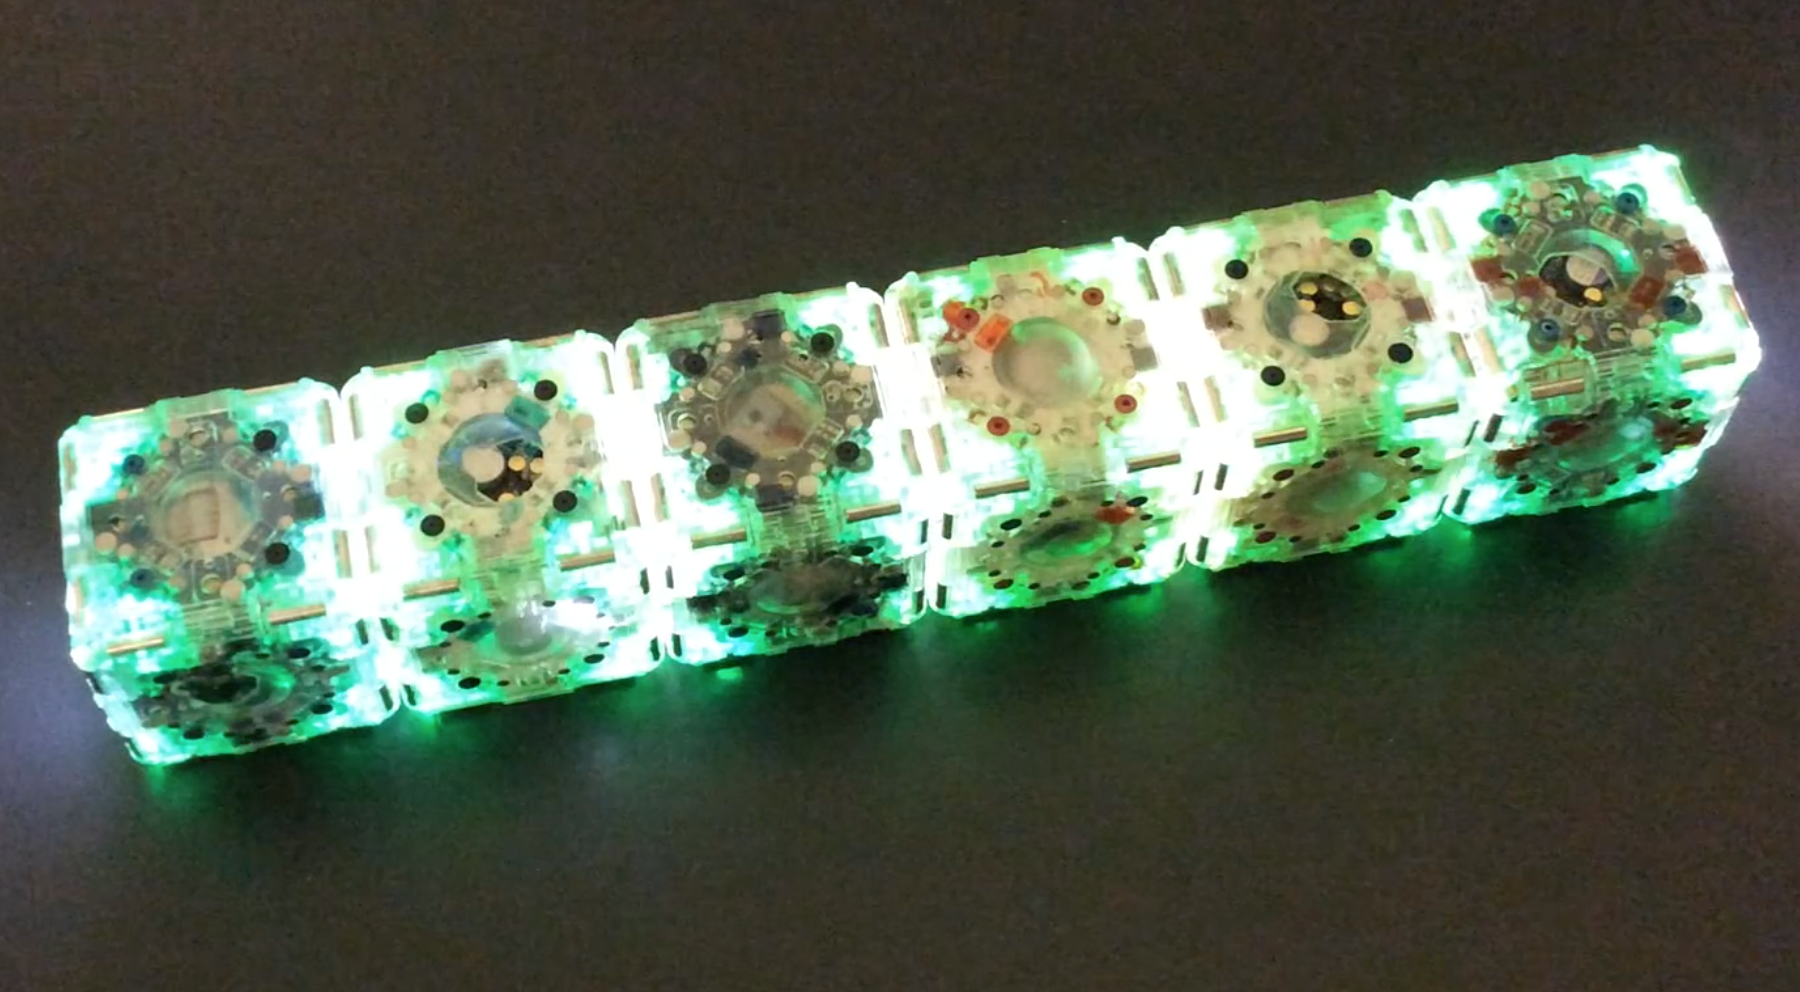
\includegraphics[width=0.9\linewidth]{figures/ActualLine_6.png}
		\subcaption{} 
	\end{subfigure}
	
	\caption{This experiment shows a random 3D configuration of M-Blocks reconfiguring into a line.}
	
	\label{fig:lineExperiment}
\end{figure}

We did experiments

%%%%%%%%%%%%%%%%%%%%%%%%%%%%%%%%%%%%%%%%%%%%%%%%%%%%%%%%%%%%%%%%%%%%%%%%%%%%%%%%%%%%%%%%%%%%%%%%%%%%%%%%%%%%%%%%%%%%%%%%%%%%%%%%%%%%%%%%%%%%%%%
%%%%%%%%%%%%%%%%%%%%%%%%%%%%%%%%%%%%%%%%%%%%%%%%%%%%%%%%%%%%%%%%%%%%%%%%%%%%%%%%%%%%%%%%%%%%%%%%%%%%%%%%%%%%%%%%%%%%%%%%%%%%%%%%%%%%%

%%%%%%%%%%
\subsection{Light guided aggregation experiments}
\label{sec:mblocksExperimentsLight}
%%%%%%%%%%%%%%%%%%%%%%%%%%%%%%%%%%%%%%%%%%%%%%%%%%%%%%%%%%%%%%%%%%%%%%%%%%%%%%%%%%%%%%%%%%%%%%%%%%%%%%%%%%%%%%%%%%%%%%%%%%%%%%%%%%%%%%%%%%%%%%%
%%%%%%%%%%%%%%%%%%%%%%%%%%%%%%%%%%%%%%%%%%%%%%%%%%%%%%%%%%%%%%%%%%%%%%%%%%%%%%%%%%%%%%%%%%%%%%%%%%%%%%%%%%%%%%%%%%%%%%%%%%%%%%%%%%%%%%%%%%%%%%%

More experiments
